\section{FPGA side}

\subsection{Introduction to some CASPER blocks}
As stated before the CASPER community created blocks that can be used in the simulink environment. The interaction of matlab-ise was supported by Xilinx and the CASPER people just extended the available blocks forming more complicated systems with the basic building blocks that Xilinx gave.

To program the FPGA we cannot use any simulink block, we need to stick to the blocks that Xilinx has or the more complex one created by CASPER. The simulink libraries that you should use are: \textbf{CASPER DSP Blockset}, \textbf{CASPER XPS blockset}, \textbf{Xilinx Blockset} and \textbf{Xilinx Reference Blockset}.

We can distinguish three types of blocks:
\begin{itemize}
    \item The blue blocks that came directly from Xilinx IPs. The figure \ref{fig:mult} shows the multiplier supplied by Xilinx. There is a $z^3$ written in the block, meaning that this multiplier will take 3 clock cycles to generate the result. Some documentation can be found \href{https://docs.amd.com/v/u/en-US/sysgen_ref}{here} or if you got luck you can search for the specific IP, like for example with the \textbf{CORDIC 4.0} although the configurations in simulink are always smaller in simulink than what the documentation says. Anyways, most of the times the documentation is not enough and the best is to simulate it.
    \begin{figure}[h]
        \centering
        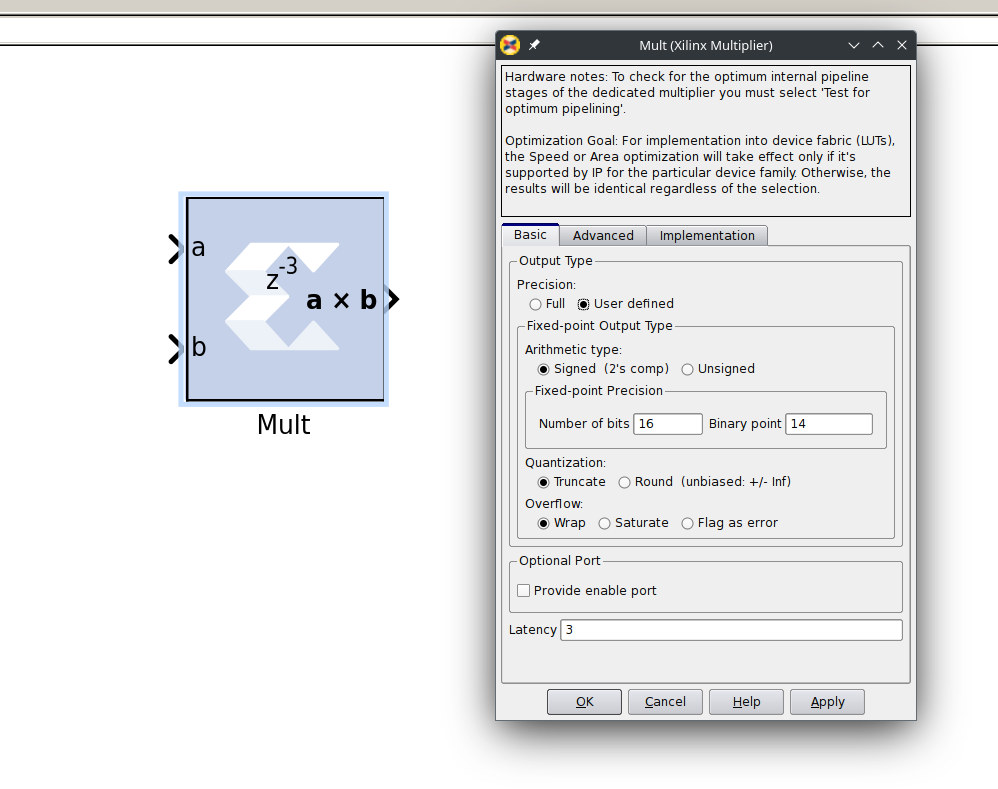
\includegraphics[width=0.7\textwidth]{images/multiplier-ex.png}
        \caption{Xilinx multiplier block.}
        \label{fig:mult}
    \end{figure}

    \item The green blocks of the \textbf{CASPER DSP blockset} are obviously DSP blocks. There you can find the FFT and the PFB among other blocks. These green blocks are created unde the hood by connecting the blue Xilinx blocks. The documentation of these blocks is not the best, you can find some documentation \href{https://casper-toolflow.readthedocs.io/en/latest/blockdocumentation.html}{here}. The figure \ref{fig:pfb_block} shows the PFB block and all the mysterious configuration fields that you need to fill (dont worry, later we will look at them). 
    There is an special type of signal that a lot of the DSP block have, the \textbf{sync\_in} and \textbf{sync\_out} signal, which is a pulse generated in given period of clock cycles to reset the internal subsytems of the block. The \textbf{sync\_in} signal has to be connected as in a daisy chain way, you just connect the \textbf{sync\_out} of the previous block with the next block. And if you need to put delays between the blocks you also have to put delays in the sync signal!!!

    \begin{figure}[h]
        \centering
        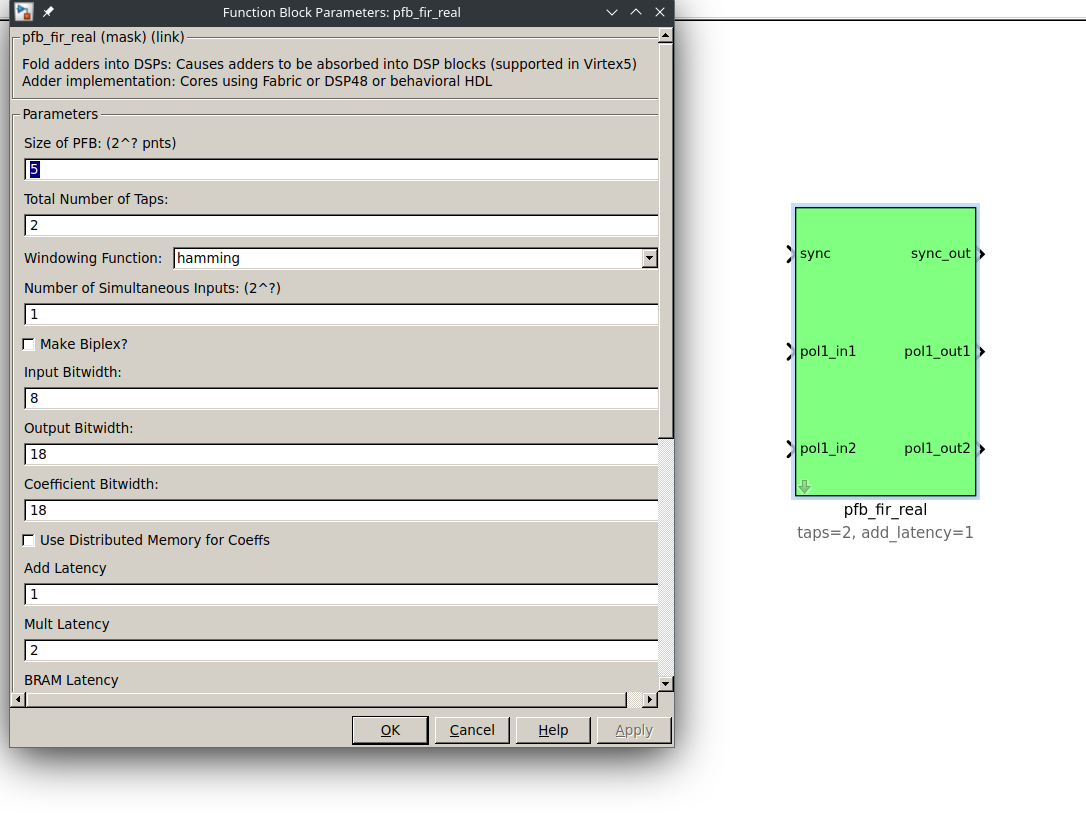
\includegraphics[width=0.7\textwidth]{images/pfb_block.png}
        \caption{PFB real block.}
        \label{fig:pfb_block}
    \end{figure}

\item The yellow blocks of the \textbf{CASPER XPS blockset}. These blocks are "special" since they are the ADC, DACs and communication blocks. The most important are of course the ADC that can be see in the figure \ref{fig:asiaa} where you can see that the ADC was configured to use 2 channels (ie it handles two analog inputs) and the sampling frequency set to 1200MHz.
    The other two important blocks are the \textbf{software registers} and the \textbf{shared brams} that are the blocks that communicate the FPGA and the PowerPC in the ROACH, enabling the configuration of the system and the readout of the state of the system.

    \begin{figure}[h]
        \centering
        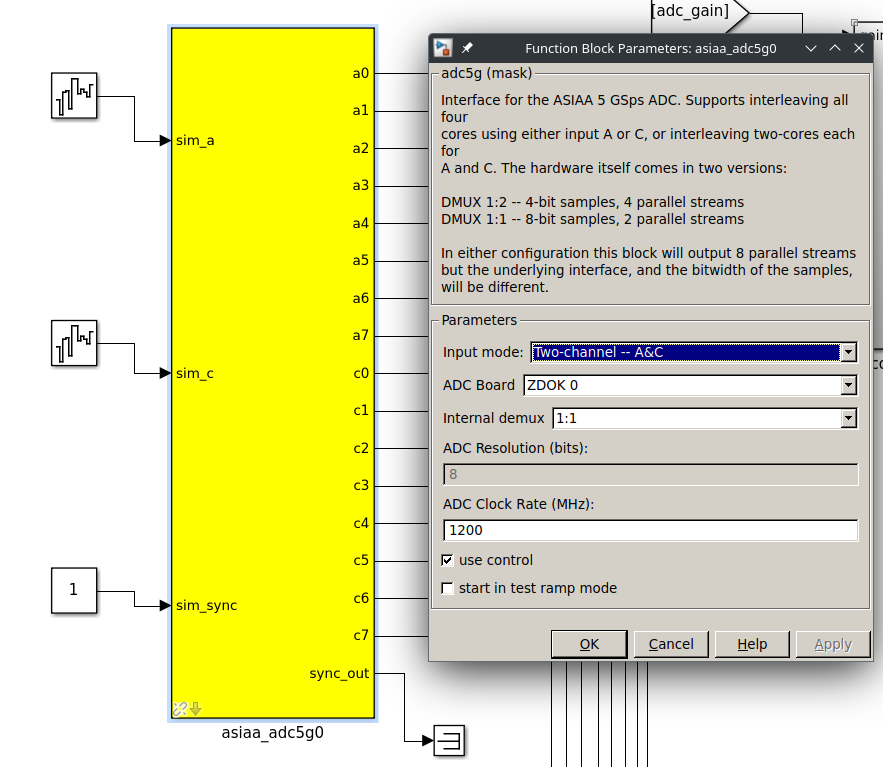
\includegraphics[width=0.7\textwidth]{images/asiaa_block.png}
        \caption{ROACH2 ADC block.}
        \label{fig:asiaa}
    \end{figure}


\end{itemize}

I cannot stress more the importance of the latency of the blocks, like for example to create a correlator we need that the data streams of both antennas have the same latency and they should arrive in a synchronous way to the multiplier, otherwise you only will obtain garbage data.


Also there are important trade-off that you should make when compiling, since the model that you are puting in simulink has to be translated to a physical location on the chip.
The best way to think about the data stream in the physical is to think of it like a guy that needs to travel from the point A to B and each block that you place is a stop in its journey. The problem arrise when the compiler needs for example to create a route between two blocks that are far away in the chip, then our traveler has to go in a single clock cycle all that distance and if he is not able the compilation will fail. The way to make this large trip is to place more stops in the way to the next destination, and this is done by adding latency in the block or to placing the \textbf{pipeline} or \textbf{delay} blocks. 

In reality the problem is not that easy, since when adding latency the compiler can decide to map the route in a different way. But thats the general idea, when not meeting timing you need to add more latency to some part of the model, but ensuring that the behaviour in the system reamins (ie you have to keep everything synchronized).

\subsection{Simulation in simulink and parametrization of the models}
As stated before the documentation is very little and most of the times the best is just to simulate the block to see how it behaves. Also, when dealing with a big system the compilations times are big, so the best is to be sure that the behaviour of your system is what you think.


To simulate in the simulink envionment you can just create a source that generates data that goes into the block that you want to test (like for example a free runing  counter) and see the outputs with an scope as the CASPER people does in \href{https://casper.berkeley.edu/wiki/Introduction_to_Simulink_ROACH2}{this tutorial} or \href{https://casper-toolflow.readthedocs.io/projects/tutorials/en/latest/tutorials/snap/tut_intro.html}{this one}. Instead of the scopes that the CASPER people showed, you can also use the \textbf{WaveScope} that allows you to look at different traces.


But this simulations are not that good, since creating a data source that generates inputs are complicated to make just using the Xilinx blocks and also we would like to have access to the output data. The ideal simulation should be to control the input data as we want and to get the output to verify that the answer to our input is what it should be.

We can feed the system with data from matlab using the \textbf{from workspace} followed with a \textbf{grateway-in} block. \textbf{From workspace} will look for local variables in the matlab session, so you can put whatever you want there and the \textbf{gateway in} block converts the sample in a fixed point one to be able to interact with the system. To get the data out you can use the \textbf{gateway out} and the  \textbf{to workspace} blocks.


The figure \ref{fig:gateway_sim} you can see that a basic simulation of the addSub block, the inputs are vectors created in the matlab environment called \textbf{dat0} and \textbf{dat1}. When running the simulation the output is written in the \textbf{simout} variable that can be accessed in matlab.
And after the simulation is run you should assert that the $simout=dat0+dat1$.

\begin{figure}[h]
    \centering
    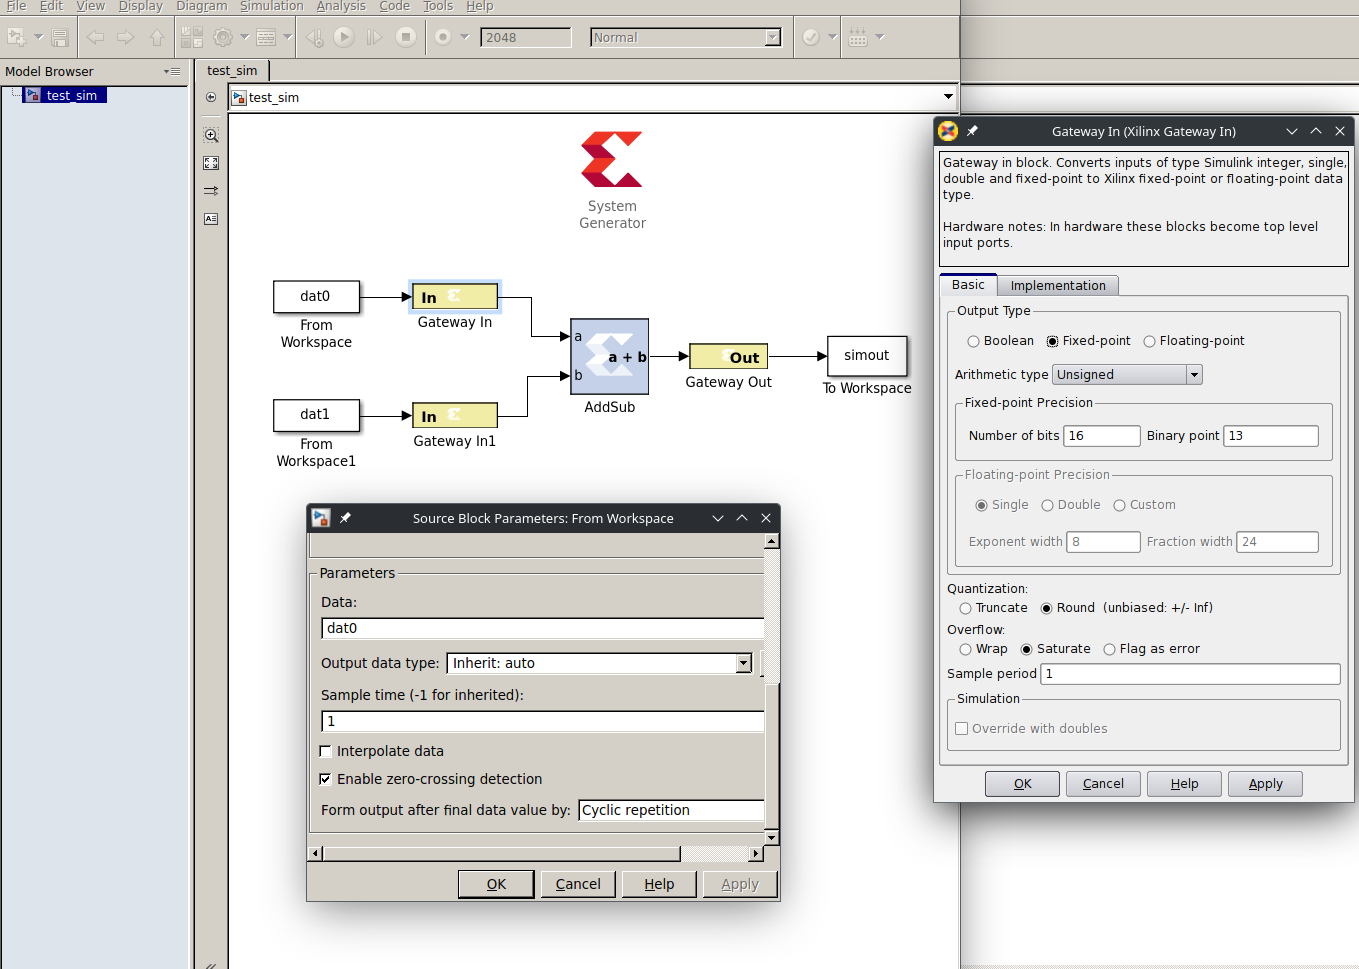
\includegraphics[width=0.7\textwidth]{images/sim_gateway_in.png}
    \caption{Simulink simulation using gateway in/out to put/get the data from the workspace in matlab.}
    \label{fig:gateway_sim}
\end{figure}

Eventually you would want to script the complete simulation, \href{https://github.com/sebajor/simulink_models/tree/master/Misc/Scripted_Simulation/simple_adder}{here} you got the simulation for this simple adder test where you just need to open the simulink model and run the s\textbf{sim\_test.m} file to make the simulation.
As example of more complicated models \href{https://github.com/sebajor/simulink_models/tree/master/Pocket_Correlators/simulation/wide_correlator_2in}{here} you have the simulation of one correlator or \href{https://github.com/sebajor/simulink_models/tree/master/Digital_Sideband_Separation/simulation}{here} you can find a simulation of a digital sideband separation that we made to have an estimated response for a theoretical front-end.


Finally, just to be super emphatic, simulate every time you can. Several of us had lost a lot of time compiling a model that doesnt work (remember, the ARTE model takes up to 5-8 hours to compile!) and that could be avoided just simulating. Also, the recomendation is to not simulate the complete project, divide it by parts and simulate them separately, otherwise you could be waiting ages because the simulink environment just sucks.

\subsection{RTL, black-boxes and cocotb}
Simulink is good if you only have to deal with DSP stuffs, when you need to make some finite state machines or anything that looks like a control system using blocks make it super complicated. Also you cannot document the thing easily, you just will see a bunch of registers and the meaning behind the states wont be clear.

Another big missed part in the simulink workflow is the incremental compilation of the subsystem. Everytime that you create a subsystem, in theory you should compile it to see what is the utilization and the expected maximum frequency that this system supports. For example if I made some math intense subsystem I would like to see that the compiler is using the embedded multipliers and not using look-up tables to make the computation, and if its not I would modify my model to use them. Also if I want to run my complete system at 150MHz and the max frequency of the compiled subsystem is 100MHz I already know that my compilation would never work and I have to put some delays here and there to improve the timming of the same block. 

In the simulink workflow you make the complete system and start to see where the timing is not meet and try to solve it after the compilation ends. Also, when looking to the big project compilated, you just lost track of how the subsystem are being translated to the physical part. 
And to add the final nail to the coffin, even we have the ability to simulate it is pain to do it in simulink.


All those reasons led me to just code some parts in verilog and simulate them verifying their right behaviour before introducing them into the simulink model.

\href{https://github.com/sebajor/verilog_codes}{Here} is the repository with my verilog codes, where for you the important directories are: \textbf{arte\_stuffs}, \textbf{casper\_utils}, \textbf{rfi\_detector} and \textbf{dsp}.
I tried to create parametrizables modules where each one has its own dedicated testbench. The testbench were made using the \href{https://www.cocotb.org/}{cocotb} library that use a python wrapper to interact with the input/output of the verilog module, then I was able to verify the correctness of every module in a incremental way.

For the most elaborated testbench I created the algorithm in python using standard libraries like numpy, and then generate a random input for the verilog module. Finally I compare that the verilog output with the python one, if the output does not match the python one the simulation ends and you could use the traces to see where is the error. 

As an example we will take a look at the \textbf{casper\_utils/tge\_write\_packetizer} that is the interface the ROACH2 10Gbe simulink block, it receives a data stream with a valid signal and it put it in the format that the 10Gbe ethernet block likes.
The interface looks as follows:

\newpage
\begin{lstlisting}[language=VBScript]

module tge_write_packetizer #(
    parameter DIN_WIDTH = 256,
    parameter FIFO_DEPTH = 512
) (
    input wire clk,
    input wire rst,
    input wire [DIN_WIDTH-1:0] din,
    input wire din_valid,
    //configuration signals
    input wire [31:0] pkt_len,          //UDP package lenght
    input wire [31:0] sleep_cycles,     //cycles to sleep after sending one package
    input wire [31:0] config_tx_dest_ip,//destination address    
    input wire [31:0] config_tx_dest_port,//destination port
    //to the TGE 
    output wire [63:0] tx_data,
    output wire tx_valid,
    output wire [31:0] tx_dest_ip,
    output wire [15:0] tx_dest_port,
    output wire tx_eof,
    output wire fifo_full
);

\end{lstlisting}

In this module we have two parameters to set when using it, the input bitsize \textbf{DIN\_WIDTH} and the \textbf{FIFO\_DEPTH} that is the amount of words that the module can handle before overflowing.

The situation is as follows, the 10Gbe block only can receive words of 64bits per clock cycle but usually we are dealing bigger words, for example an usual 4 lane spectrometer will generate 256bits per clock cycle, so we created a FIFO to store the 256bits words and read them in 64bits chunks. As the reading will take more cycles than the writing, depending on the period of the valid input signals and the value of the \textbf{FIFO\_DEPTH} we could end up overflowing the FIFO. But the good new is that we are able to simulate that easily using cocotb.


The code structure is always similar, there is a:
\begin{itemize}
    \item \textbf{module.v}: This is the implementation of the desired subsystem.
    \item \textbf{module\_tb.v}: This is the instantiation of the module. Some times it has some glue logic to make the interface with python easier, but most of the times just sets the hyperparameters (although there are some more advanced testbench where also the hyperparameters are explored).
    \item \textbf{module\_test.py}: Here is the testbench itself. The data is created and feed into the \textbf{module\_tb.v} while another thread is reading the outputs to check the correctness of the model. For the case of the \textbf{tge\_write\_packetizer.v} its checking that 64bit data sent to the 10Gbe block match the 256bits portion written to the input. Also it checks that the signal timming is correct and that the FIFO is not overflowing.
    \item \textbf{Makefile} This file is used to run the testbench, to create the signal traces report and to clean the products of the simulation. To just run the simulation you have to issue \textbf{make} and this will tell you if the system was able to pass the test or if it fails. To get the traces you should run \textbf{make WAVES=1}, in this case when the simulation stops you should get a trace file called \textbf{traces.fst}, so if the system fails in one clock cycle it will ends there and you can trace back the problem. Finally if you run \textbf{make clean} all the subproducts will be erased.

\end{itemize}

For this test I want the system to fail so I put \textbf{FIFO\_DEPTH=32} and start the simulation with \textbf{make WAVES=1} and I got the output shown in the figure \ref{fig:cocotb_fail} and opening the traces in figure \ref{fig:cocotb_trace} we can see that indeed the signal called \textbf{fifo\_full} was raised. If there is no error in the module, after the \textbf{make} command you will see that all the test were passed.

\begin{figure}
    \centering
    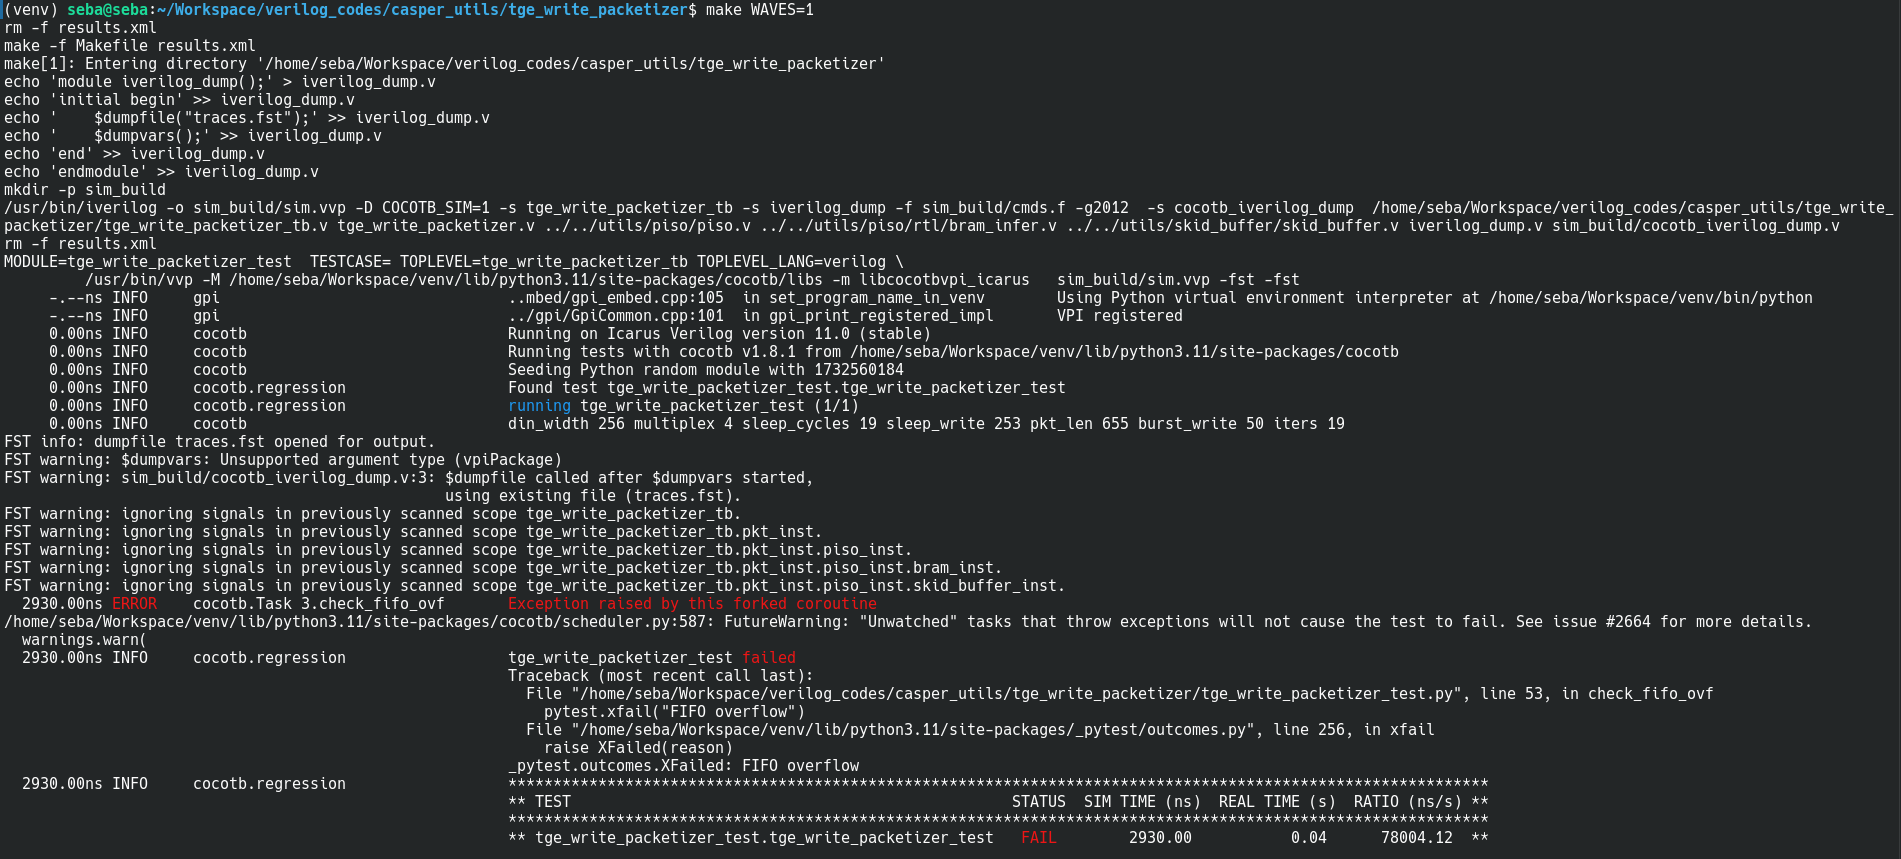
\includegraphics[width=1\textwidth]{images/cocotb_out.png}
    \caption{Fail test. The simulator report that the fail was due a FIFO overflow.}
    \label{fig:cocotb_fail}
\end{figure}


\begin{figure}
    \centering
    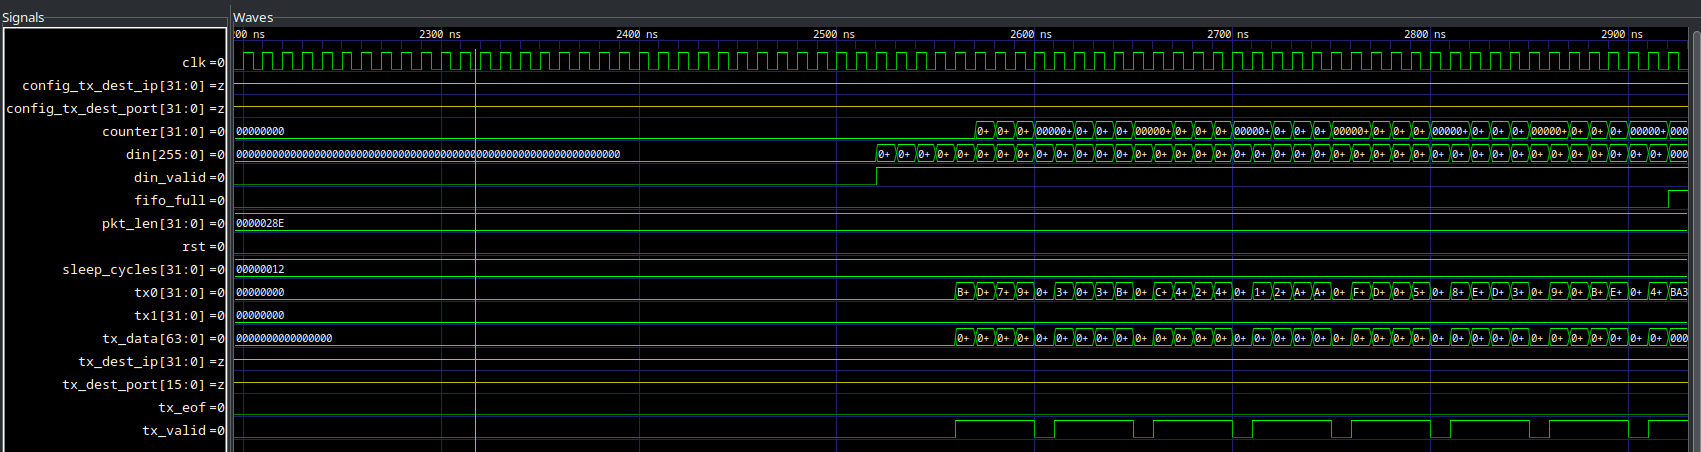
\includegraphics[width=1\textwidth]{images/gtk_traces.png}
    \caption{Generated traces for the failed simulation.}
    \label{fig:cocotb_trace}
\end{figure}


Maybe you still dont get why I insisted that much on this kind of simulation so here goes my two cents:
\begin{itemize}
    \item If you show that your system worked as intended with random inputs then it will probably work out of the box when putting it in the FPGA.
    \item You can study the bitwidths effects over the algorithms. For example, if you collect real data you can feed it to the algorithm and find the best representation that does the job.
    \item When failing you have access to all the traces. If you try to debug the system on hardware you can access to some portion of them and you have to be able to decipher the status of the system.
    \item Having the testbench traces is a kind of documentation helper, since you can see the timing of the signals that the modul expect. \footnote{Although they should be documented anyways, if not its my bad.}
    \item Once you probed the modules you can keep usign them without worrying if they will fail in some edge cases (in theory you have to tested agains random data, so it should have meet some weird cases).
    \item The simulation is way more faster than the simulink one.
    \item When having ready the module you can compile it and review the expected maximum frequency and the resource usage.
\end{itemize}

The biggest issue with this is that since the Xilinx peoples are assholes they hadnt open their simulator, so you only can simulate verilog code. Then all their IPs blocks cant enter to the simulator.




\subsection{DRAM ring buffer}
This is the perfect example of why we all got tired of simulink and I started to look for alternatives (sorry if that makes your life more complicated).

The DRAM in the ROACH2 is a 1.125GB module and for a long time was unusable since the CASPER block was broken and did not work. Luckily I got \href{https://www.mail-archive.com/casper@lists.berkeley.edu/msg08146.html}{help} from some fellow casperite, finally I put the changes in \href{https://github.com/sebajor/mlib_devel}{this repository}, but with the following caveats: First we cannot use the \textbf{.bof} files, we need to use the \textbf{.fpg} files, and second the ROACH needs to have an updated kernel (they came with an old one). In the installation section I placed a link with the guide to do the kernel update.



The DRAM ring buffer subsystem consist on three parts:
\begin{enumerate}
    \item Bit reduce: since we are running the ADCs at 1200GSa/s and we have 8 samples per clock cycle we are running the FPGA at 150MHz. For this ADCs we have that each sample has 8bits so we are generating 1.2GB/s per channel and we want to save 3 channels in a ring buffer. This means that we are dealing with 3.6GB/s. Since our DRAM has 1.125GB we will be able to save $1.125GB/(3.6GB/s)=0.3125s$.  Like this is a small timeslot we decided just to save 4bits of the samples to double the time that we have in the ring buffer.
        To make this we use a multipler to add digital gain to the samples as the figures \ref{fig:gain_block}, \ref{fig:gain_block1} and \ref{fig:gain_block2} shows. The normal behaviour is to represent the ADCs samples as signed samples with 8 bits and the binary point at the bit 7, then we multiply by a \textbf{gain} value that is represented as signed 32 bit with the ninary point at the bit 10, from the resulting output of that multiplication we only keep a signed sample of 4 bits without  binary point.
 I put also a snapshot to get the reduced samples of the ADC0 as the figure \ref{fig:reduced_snapshot} shows, there you can compare the input data spectrum with the reduced one. I made \href{https://github.com/sebajor/ARTE-control/blob/main/codes/dram_bit_usage.py}{this code} to plot both real time spectrums just to check. My recomendation here its to save the some raw ADC data and check the actual gain that you need, simulate the stuff with real sky data. 


    \begin{figure}
        \centering
        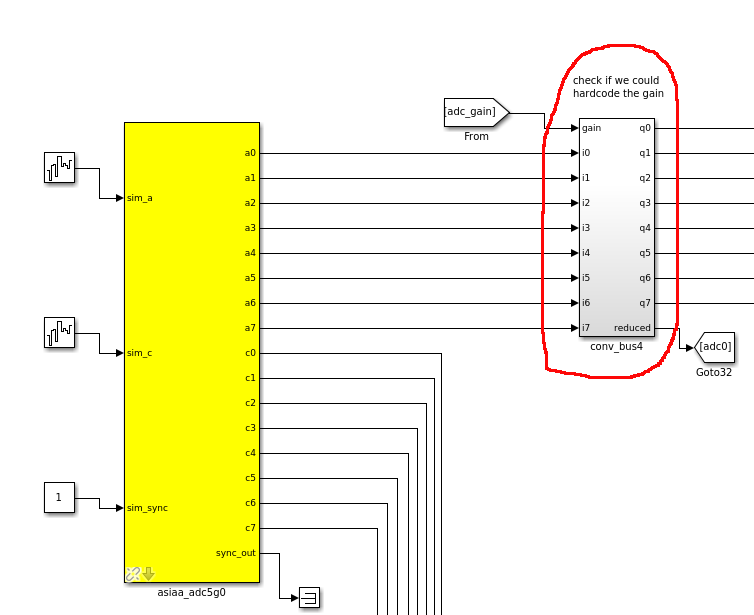
\includegraphics[width=0.7\textwidth]{images/adc_and_gain.png}
        \caption{Bit reduce Top view. In red is the submodule where the bit reduction occurs.}
        \label{fig:gain_block}
    \end{figure}
    \begin{figure}
        \centering
        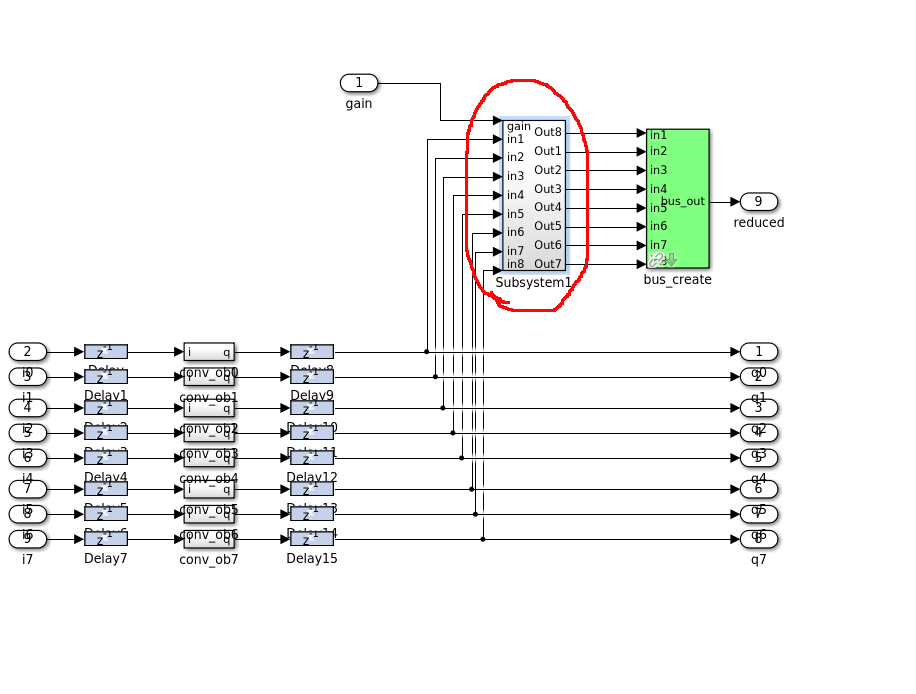
\includegraphics[width=0.7\textwidth]{images/adc_gain1.png}
        \caption{Bit reduce first level of the block. Here all the samples are converted from unsigned to signed, one path leads to the output that goes into the PFB and the output called \textbf{reduced} goes to the DRAM.}
        \label{fig:gain_block1}
    \end{figure}
    \begin{figure}
        \centering
        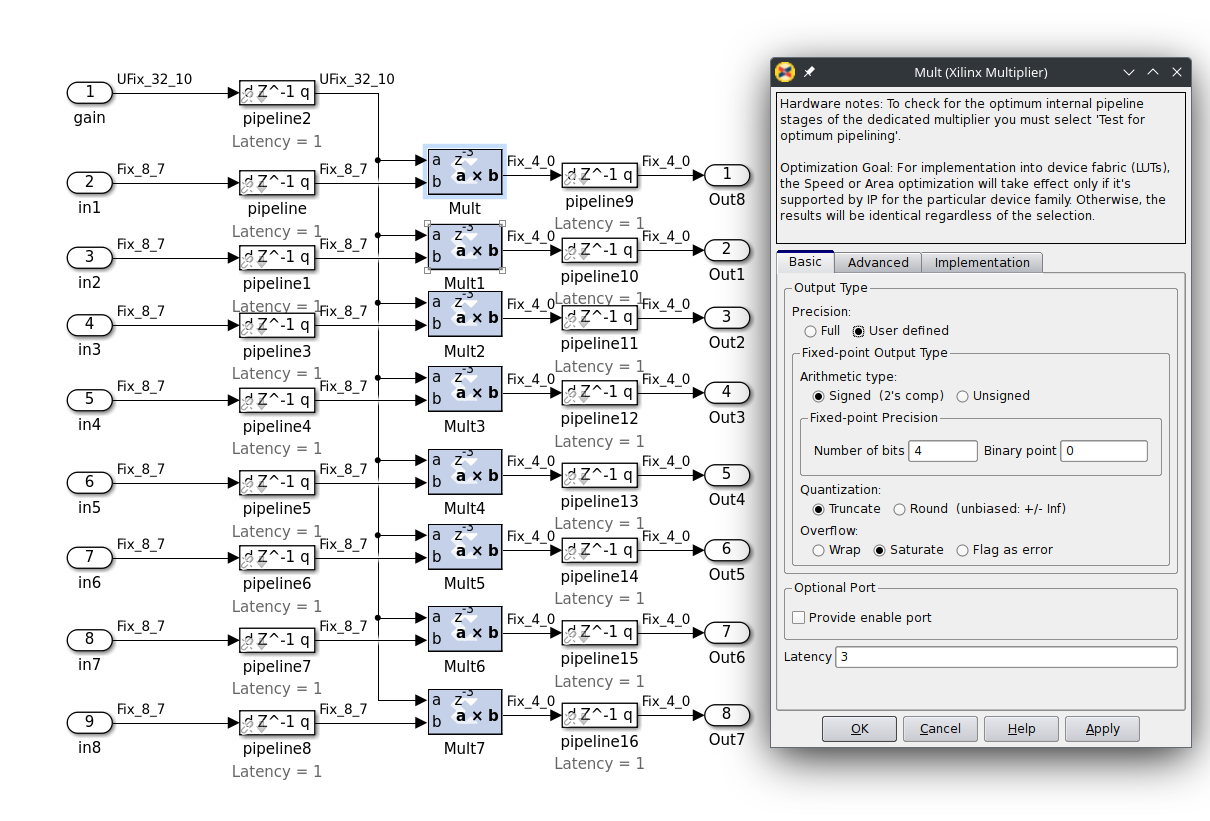
\includegraphics[width=0.7\textwidth]{images/adc_gain2.png}
        \caption{Bit reduce second level of the block. The ADC signal arrives with 8 bit and the point at the bit 7, after the multiplication by a gain that is a 32 bits with the bit point at 10 we output a 4 bits sample without binary point. So you have to give the best gain value that represent your data.}
        \label{fig:gain_block2}
    \end{figure}


    \begin{figure}
        \centering
        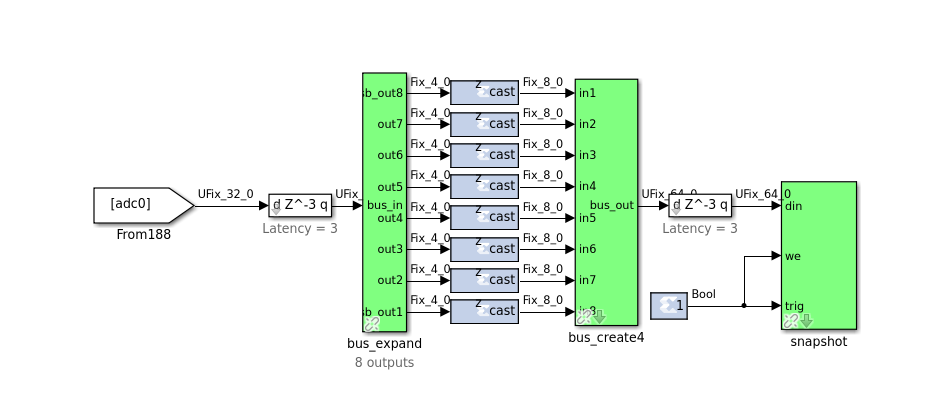
\includegraphics[width=0.7\textwidth]{images/dram_snapshot.png}
        \caption{DRAM bit reduced snapshot. You can compare the read values with the non-reduced snapshot.}
        \label{fig:reduced_snapshot}
    \end{figure}


\item DRAM interface: The interface of the DRAM is \href{https://casper.astro.berkeley.edu/wiki/Dram}{Here}. Again we have $8samples/cycle*3streams = 8*(4bits)/cycle*3 = 96bits/cycle$ and the DRAM words are of $288bits$, so we need to join $288bits/(96bits/cycles) = 3cycles$ of data before sending the data into the DRAM. Also if you read the documentation of the interface of the DRAM you will see that you need to create a given behaviour (like having the signal \textbf{cmd\_valid} low for two cycles, etc), all this was made just using counters and some black magic boolean logic and it does the job. Since when I did this model I was just using simulink I cannot gave you traces or something like that to decipher whats going on but I will make my best to explain the bigger picture. The external view of this subsystem is at \ref{fig:dram_external} and the internal view is at \ref{fig:dram_internal}
    \begin{enumerate}[label=(\alph*)]
        \item Inside the ring block we have an internal configuration registers where you can set the action of the DRAM (read or write) and also has some reset signals. The controls signals are shown in the figure \ref{fig:dram_control}. We have another register that are used only in the read mode. When reading the data from the DRAM we want to do it in burst mode, that means we need to read several addresses otherwise the latency will be higher this is controlled by the register called \textbf{n\_pkt}. And lastly the third register is to configure the amount of cycles that the system will sleep after one burst read, this is because of two reasons: you can overflow the FIFO that receive the DRAM data and because if you read the data too fast and send it to a computer you can start to loose packages. The lost of packages is because the computer is not able to get all the data that the FPGA is sending. Even if I did the stuff I cannot give more info (this is why I hate simulink)... when interfacing the control signals I made a python class that hides the inside complexity, you better just use it. The class is \href{https://github.com/sebajor/ARTE-control/blob/main/codes/dram_class.py}{here}.
        \item The writing part accumulate three clock cycles of data, and when is ready it  gives it at the DRAM in the format the blocks like (holding \textbf{cmd\_valid} signal down and keeping the address fixed). To start write the internal write command and the external write port should be both high, otherwise it stops the writing and keep the address fix, this is the method to stop the writing if there is a detection.
        \item The read part starts to work when the internal read control signal is set to high. The read part has its own address counter that is added to the write one to start reading the data in the same point that the writting part ended to write to. As mentioned previously in this mode the reading is being done in a burst mode, where you ask for several addresses and after an unknown number of cycles you will get the response \footnote{Yes, you read it right, the DRAM reading is not deterministic} with a valid signal.
        \item Since we read the data in a bursty mode then we store the data in a FIFO that will be later read in smaller chunks. Since we use the 1Gbethernet port to send the data we use an HDL that does the job of taking a word of 288bits and delivers an 8 bit word. And again we have some black magic to generate the data frame that the 1Gbe block likes and also holding the sleep cycles that you set to not saturate the computer buffers.
    \end{enumerate}


    \begin{figure}
        \centering
        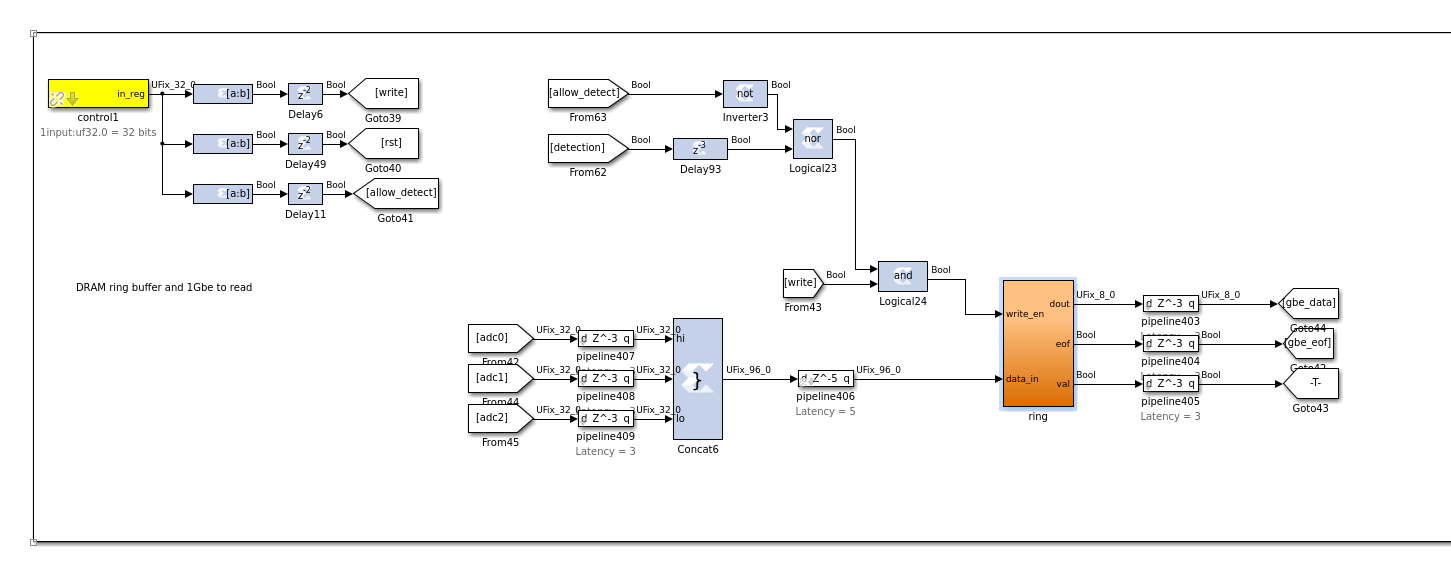
\includegraphics[width=0.7\textwidth]{images/dram_ring_buffer.png}
        \caption{External view of the DRAM ring buffer subsystem. It receives the inputs from the 4bits-ADC samples and a write enable signal that is disabled by the some detection signal.}
        \label{fig:dram_external}
    \end{figure}

    \begin{figure}
        \centering
        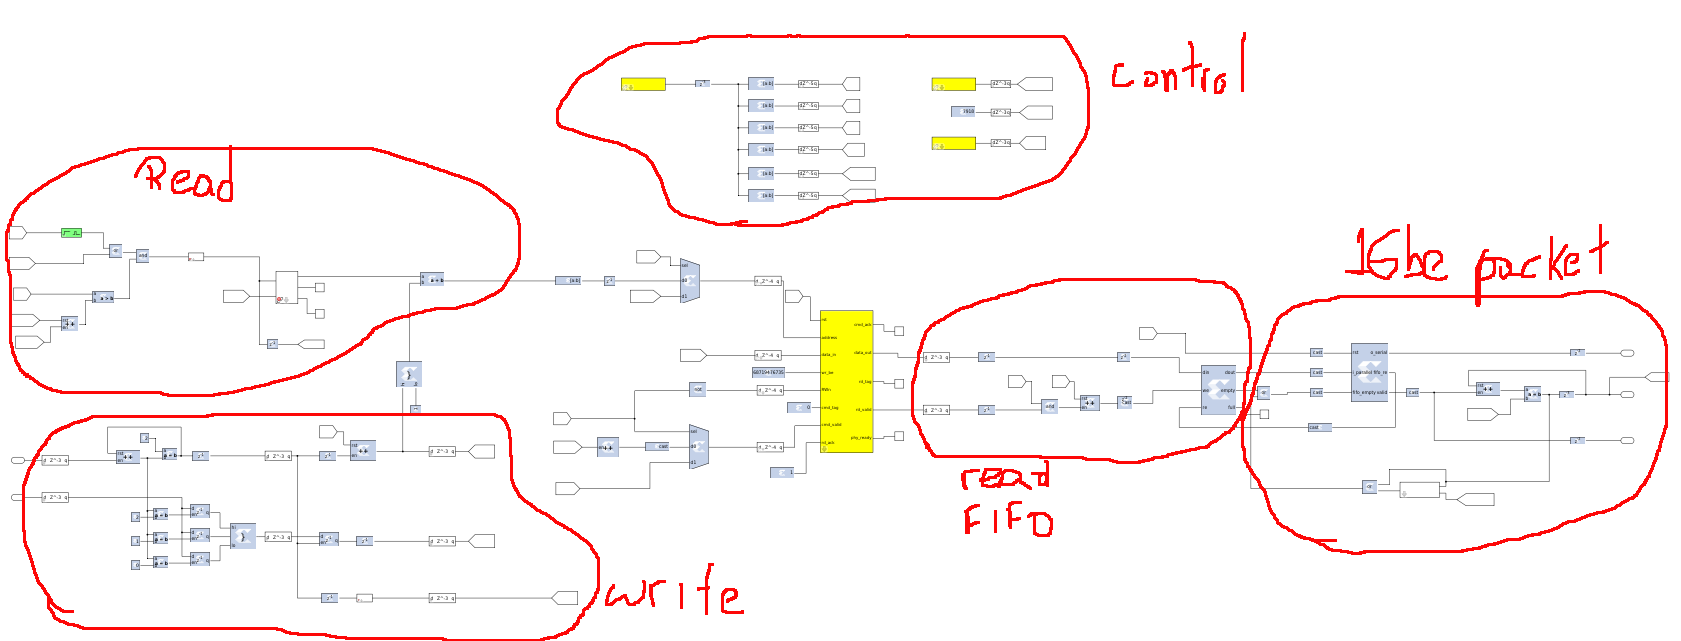
\includegraphics[width=0.7\textwidth]{images/dram_ring1.png}
        \caption{Internal view of the DRAM ring buffer. There are mainly 4 subsystem here: write, read, control, read FIFO and the 1Gbe packetizer.}
        \label{fig:dram_internal}
    \end{figure}

    \begin{figure}
        \centering
        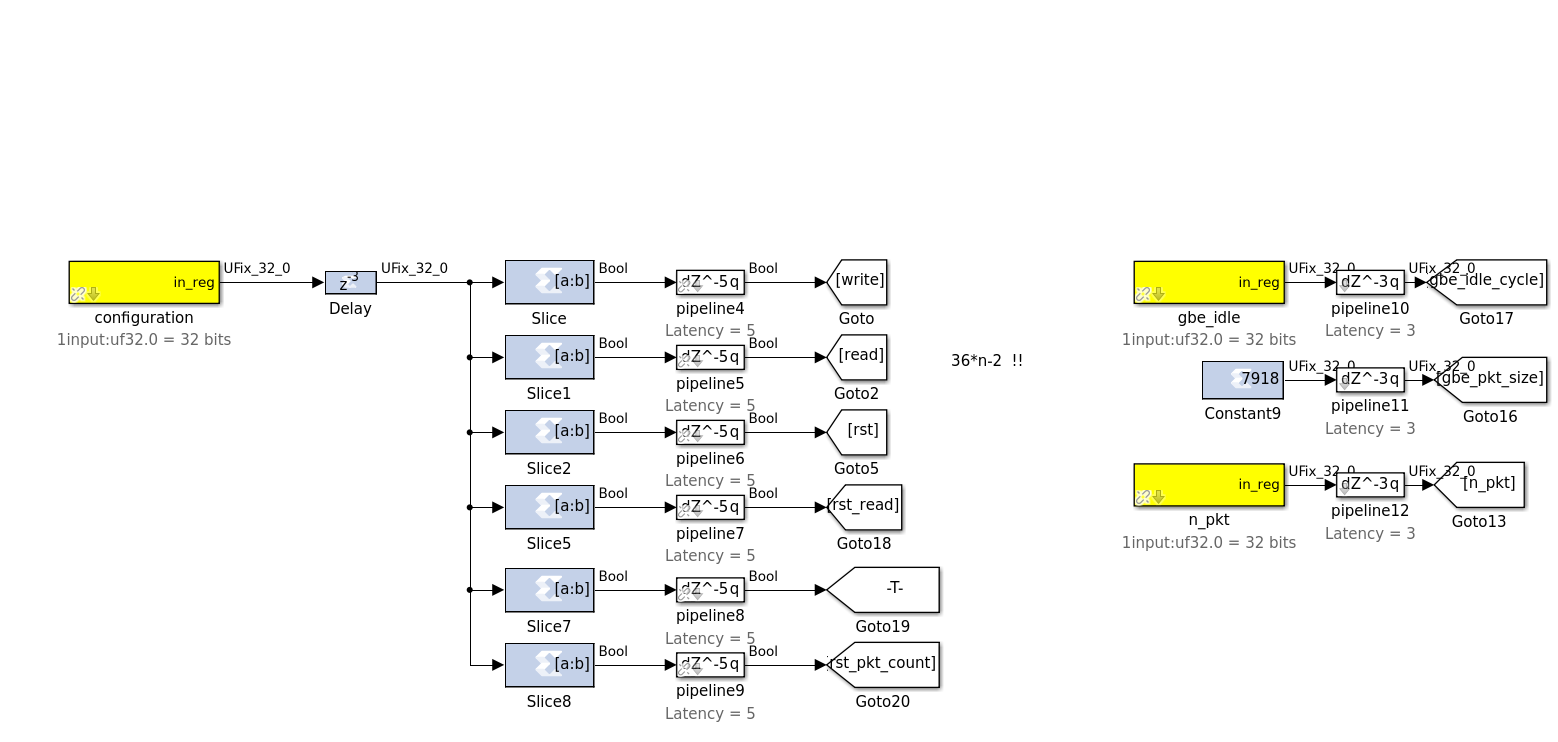
\includegraphics[width=0.7\textwidth]{images/dram_ring_register.png}
        \caption{Internal control signals for the DRAM ring buffer.}
        \label{fig:dram_control}
    \end{figure}

\item The last part of the ring buffer is the interface between the DRAM and the ethernet port, that you can see in the figure \ref{fig:dram_ethernet}. This is the ethernet port that is connected to the FPGA, so in principle as long as you feed data to it, it will send it even if the computer is not able to follow it. The other problem that adds up is that as this interface is controlled by the FPGA it doesnt has a complex control system and just send UDP packages, so if the packet got lost you are in charge of notice that and ask the system to send the lost packet. This logic it is not implemented, so you have to be carefull how fast you send the data (this is controlled with the \textbf{gbe\_idle} internal control signal.
     \begin{figure}
        \centering
        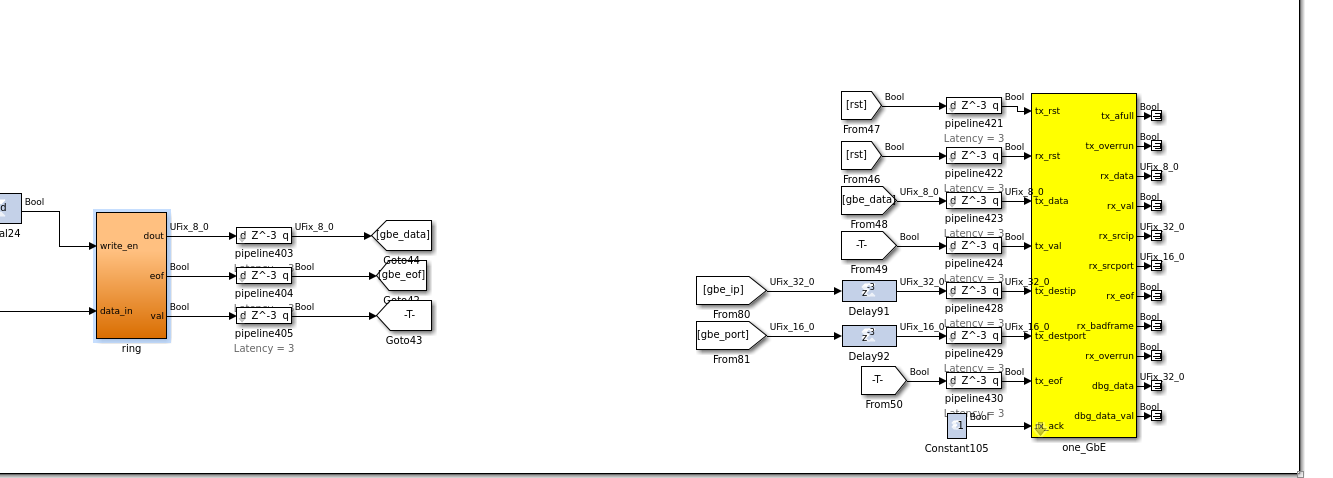
\includegraphics[width=0.7\textwidth]{images/dram_final_view.png}
        \caption{Ring buffer connection to the ethernet block.}
        \label{fig:dram_ethernet}
    \end{figure}

    \item Finally, there is another problem with this subsystem... If you try to compile a model with the 1Gbe port and has some resource usage, it will surely fail to meet timing. This is because the ethernet port has a fixed location in the chip, so when the compiler tries to generate the primitives it can put the ethernet block related parts far away of the physical location. The solution is to create a constrain in the offending modules to force the compiler to put them in a nearby region, in the CASPER toolflow this is done by using a UCF as the figure 

     \begin{figure}
        \centering
        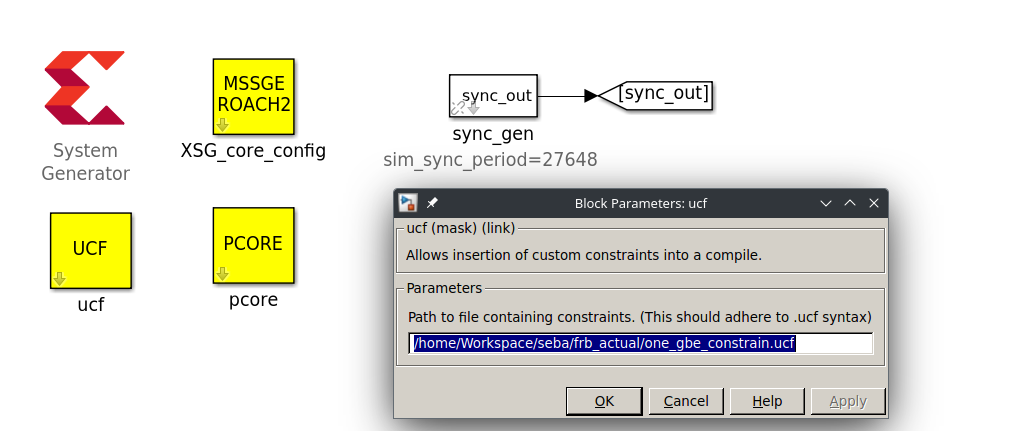
\includegraphics[width=0.7\textwidth]{images/eth_ucf.png}
        \caption{User constrain file}
        \label{fig:ucf}
    \end{figure}
    The \textbf{"one\_gbe\_constrain.ucf"} has the following content:

    \begin{lstlisting}
INST "arte_one_GbE" AREA_GROUP = "pblock_arte_one_GbE";
AREA_GROUP "pblock_arte_one_GbE" RANGE=SLICE_X168Y153:SLICE_X205Y179;
AREA_GROUP "pblock_arte_one_GbE" RANGE=DSP48_X11Y62:DSP48_X13Y71;
AREA_GROUP "pblock_arte_one_GbE" RANGE=RAMB18_X11Y62:RAMB18_X13Y71;
AREA_GROUP "pblock_arte_one_GbE" RANGE=RAMB36_X11Y31:RAMB36_X13Y35;
    \end{lstlisting}

    As you note the ucf uses the name \textit{arte} in several parts, this is because when compiling the complete model it uses the name of the simulink system to create the netlists.. This means that if you copy and paste the model in other place you should keep the name as \textit{arte.slx} or the constrain wont work (or you can also edit the ucf accordingly). I know that there are best ways to write the UCF (the 10Gbe block has its own ucf) so you can check how to do it better.


\end{enumerate}

When I started this section I said that this is the best example of how horrible can be the design in simulink and now that you have gone through it I think you should agree. There are some magic numbers here and there that myself dont know where I took them and if you change them maybe the system breaks. I started to code the new interface to the DRAM block \href{https://github.com/sebajor/verilog_codes/tree/main/casper_utils/dram_intf}{here}. I also start to make one interface to handle the automatic reading of the DRAM and send the data via the ethernet block \href{https://github.com/sebajor/verilog_codes/tree/main/casper_utils/work_in_progress/dram_one_gbe}{here}, and \href{https://github.com/sebajor/verilog_codes/tree/main/casper_utils/work_in_progress/dram_tge}{here} I started the same automatic reading but then interfacing the 10Gbe port, but I did not test the modules in the actual hardware so I am not sure of the behaviour (but there are at least some simulations).



If you have time, I recommend to change the DRAM ring buffer finishing the verilog implementation that I started. Even if it now does the job, it can not be maintained and its pure black magic, but I would say that is not a high priority task.















\subsection{PFB and FFT}

\subsection{Beamforming}

\subsection{10Gbe spectra data acquisition}

\subsection{DoA}

\subsection{RFI detection}

\subsection{Channel flagging}

\subsection{Dedispersion}

\subsection{FPGA control subsytem}

\subsection{Hyperparameters}



This was one of my good ideas, but sadly I didnt encourage its usage and now it ends up being just an non-updated document. 



\subsection{Timestamp}





